%%%%%%%%%%%%%%%%%%%%%%%%%%%%%%%%%%%%%%%%%%%%%%%%%%%%%%%%%%%%%%%%
\begin{comment}

* Maintain 80 characters / line.
 
* too much ``''s make the sentence look scattered and visually less recognizable. ``e.g.'' also.

* \em, \bf, \it are all obsolete \TeX primitives, and it does not take effect properly --- for example, {\bf {\it aaa}} shows ``aaa'' in italic but NOT IN BOLD. Use \emph{}, \textit{}, \textbf{} and so on.

* always use \ff, \fd, \cea, \pr, \mv , and do not use it directly, e.g. FF, FD/LAMA2011, etc. 

* use of footnotes should be minimized.

* IPC2011 should always be \ipc . The definition can later be modified in abbrev.sty .

* prefer separated words over hyphened words. domain
  independent>domain-independent, planner independent >
  planner-independent.

* Table, Figure, Fig., should not be used directly. Always use \refig and \reftbl. When the development flag is enabled, direct use of \ref signals an error.

* Caption ends with a period.
\end{comment}

%%%%%%%%%%%%%%%%%%%%%%%%%%%%%%%%%%%%%%%%%%%%%%%%%%%%%%%%%%%%%%%%

\begin{abstract}
% % intentionally made different from the 1st-order symbol paper, writing style is also different
% While domain-independent classical planning is an active area of research,
% its applicability to the real-world tasks are limited to those precisely modeled by human.
% Recently, \latentplanner \cite{Asai2018} combined classical planning with deep-learning
% to obtain the symbolic description of the image based domain.
% In this paper, we address a problem in their preliminary implementation of \latentplanner,
% specifically the uninformative / random propositions in the latent / symbolic encoding,
% and provides a remedy for it.
% %
% Those uninformative propositions become true or false depending on the coin flip,
% which means that
% % some of the propositiosn in the latent layer may not carry significant meaning / affect the output.
% % While this is not problematic for encoding/decoding, from search/planning perspective this is a major problem,
% % because this means that 
%  a single state can have multiple propositional representations and no longer the
% unique representation amenable for search algorithms.
% % 
% One effective way to suppress this behavior is to have an additional regularization
% for the latent propositions which guides the training so that 
% % toward sparser, disentangled propositional representation,
% unused propositions tends to be 0.
%  % 
% We empirically show that this ``Zero-Suppressed SAE''
% has lower variance encoding (more stable propositions) for each single state
% and improves the success rate of \latentplanner.
% % XXX TODO: unknown if it is possible
% [TODO]
% Furthermore, we show that this Zero-Suppressed SAE can act like a declarative knowledge base
% where you incrementally assign new knowledge to unused propositions.
% We show this by retraining an existing network
% with a mixture of the existing and new dataset, and demonstrating that
% it can encode both environments.

While Classical Planning is one of the oldest active branches of AI,
its applicability is limited to the tasks precisely modeled by human.
Fully automated high-level agents should be instead able to find a symbolic representation
of an unknown environment without supervision, i.e., no help from
manually-assigned labels nor predefined reinforcement signals,
otherwise it exhibits knowledge acquisition bottleneck.
% 
Meanwhile, \latentplanner \cite{Asai2018} uses a Neural Network
called State AutoEncoder (SAE) to obtain a propositional
representation of the image based puzzle domains unsupervised,
and performs Classical Planning on the propositional state space discovered,
partly resolving this bottleneck.

In this paper, we propose a new sub-problem of symbol grounding problem (SGP)
that was not identified until SGP materialized in \latentplanner, namely
the symbol \emph{stability} problem.  Informally, symbols are
\emph{stable} when they refer to the same concept for the exact same
observation of the environment, and unstable symbols are harmful for symbolic
reasoning.
 % 
We identify that the propositional symbols found by \latentplanner 
are largely unstable with a wrong set of hyperparameters.
% 
To address this issue, we propose ``Zero-Suppressed SAE''
(ZSAE), an enhancement of SAE that uses the idea of closed-world
assumption as a strong prior for neural network optimization 
and robustly generates a set of stable symbols.
 % 
We empirically show that it finds more stable propositions
against various hyperparameters and improves the success rate of
\latentplanner.
\end{abstract}


\section{Introduction}

% [This second version of introduction is too long]

Symbol Grounding Problem (SGP) \cite{harnad1990symbol,Steels2008} is one of the key milestones in AI research
which seeks to achieve high-level intelligence beyond reflex.
In Physical Symbol Systems Hypothesis \cite{newell1976computer}, it is believed that
an agent with high-level intelligence performs tasks by efficiently manipulating a compact set of abstract symbols.
% 
Symbolic manipulation consists of mechanical applications of composable rules which allows for
development of highly optimized and generalized, domain-independent heuristics (e.g. FF \cite{Hoffmann01} or LMcut \cite{Helmert2009})
that can be easily applied to multiple tasks with few or no data,
while the current learning-based approaches struggle to improve its multi-task performance and data efficiency.
For example, training AlphaGo \cite{alphago} takes days on a huge cluster of custom-made Tensor Processing Units.
% 
To enable such a fully automated high-level symbolic computation in a real-world environment,
agents should be able to find the symbolic representation of the environment by itself, i.e. solving the Symbol Grounding Problem.

Recently, Latplan system \cite[\refig{fig:overview}]{Asai2018} successfully
connected a subsymbolic neural network system and a symbolic Classical Planning system
to solve various visually presented puzzle domains.
% In contrast to the work by Konidaris et. al. (\citeyear{KonidarisKL14}),
% Latplan is a straightforward NN built upon a \lsota framework.
The State AutoEncoder (SAE) neural network in \latentplanner
generates a set of propositional symbols from the training data consisting \emph{only of images},
i.e., by unsupervised learning without manual tagging,
and provides a bidirectional mapping between images and propositional states.
% 
The system then solves the propositional planning problem using a classical planner Fast Downward \cite{Helmert04}
and returns an image sequence that solves the puzzle
by decoding the intermediate propositional states of the plan.
It also discovers a set of action symbols that distinguish the modes of
state transitions through AMA$_2$ unsupervised learning process.
Therefore, the system solves SGP for two kinds of symbols:
Propositional symbols and action symbols.
% 
The system opens a promising direction for
applying a variety of symbolic methods to the real world, \emph{not just planning}:
In fact, the search space generated by \latentplanner was shown to be compatible
to an existing Goal Recognition system \cite{amado2018goal}.

However,
neural networks in general do not have a strong guarantee on the learned results,
and thus the propositional representations learned by Latplan have a problematic behavior.
The propositional symbols generated by Latplan are not always
``stable'', i.e., some propositions may not remain true or false given the same image input
and rather flip randomly.
These \emph{unstable} propositions do not affect the output image decoded from the propositional state either.
Thus they are ``unused'' and ``uninformative'' at the same time.

Unstable symbols are harmful for symbolic reasoning because
they break the identity assumption built into the reasoning algorithms.
For instance, in \latentplanner, 
a single image may map to multiple propositional states due to stochasticity,
therefore the duplication detection in search algorithms such as \astar \cite{hart1968formal}
cannot detect that a single real-world state is visited multiple times through
different symbolic state representations.

This problem arises for any grounding processes that do not explicitly tries to stabilize the
representation of the environment.
The first contribution of this paper is the definition of a sub-problem of symbol grounding
called ``symbol \emph{stability} problem'', which seeks to find a set of stable symbols
when the grounding procedure is non-deterministic.

The second, and more concrete, contribution of this paper is
the proposal of Zero-Suppressed State AutoEncoder (ZSAE, \refig{zsae-overview}), an enhancement of SAE in \latentplanner
that has an additional regularization penalty function for the neural network 
that makes the learned propositions more ``stable''.

ZSAE addresses three issues in the original Latplan.
The first two issues are directly related to the unstable symbols.
Unstable symbols affect search algorithms in two ways:
First, they increases the number of node generations because
it confuses the duplicate detection mechanism.
Second, and more important, issue is that they may make the state space graph disconnected because certain edges
are connected to only one random variant of the symbolic representation of real-world states.
This makes planning to fail without solution or return a suboptimal or even wrong solution.
% In fact, in the appendix section in the Arxiv version of the original paper \cite{Asai2018},
% the authors stated that they used \emph{state augmentation} technique
% which circumvent this problem by sampling states from the same image multiple times.
Thirdly, the system is sensitive to the hyperparameter, and with an inappropriate set of parameters
the propositional symbols are highly unstable.
Specifically, if we set the number of propositions ($=$ number of nodes in the latent layer) too high, the network
has an excessive capacity which results in too many unused, unstable propositions.

\begin{figure}[htb]
 \centering
 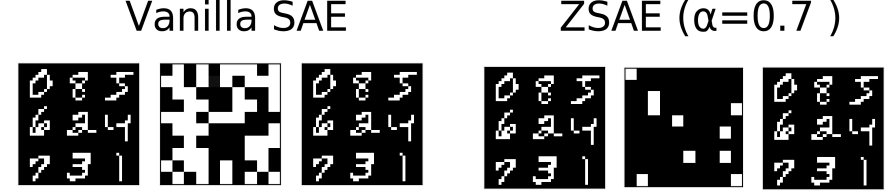
\includegraphics{img/zsae-overview.pdf}
 \caption{
Example of Vanilla SAE and Zero-Suppressed SAE (ZSAE) autoencoding a MNIST 8-puzzle state, with 100 propositions.
ZSAE obtains a representation that has fewer true bits.}
 \label{zsae-overview}
\end{figure}


% To address these problems,
% we introduce an additional regularization penalty function for the neural network 
% that makes the learned propositions more ``stable''. In the resulting neural network,
% Zero-Suppressed State AutoEncoder (ZSAE, \refig{zsae-overview}), this penalty function
% guides the network optimization so that unused propositions tend to 
% take the value of zero (false) instead of random values,
% resulting in a more stable representation.
% The stability can be measured by taking the variance of the representation from the same set of inputs.
% We also show that a more stable representation results in a higher success rate of classical planning.
% 
% Also, with this additional penalty, the number of bits required to represent the same function
% is minimized and the network becomes less sensitive to the hyperparameters.

In Zero-Suppressed SAE (ZSAE), an additional penalty function
guides the network optimization so that unused propositions tend to 
take the value of zero (false) instead of random values,
resulting in a more stable representation, measured by the variance of the representation from the same input.
The stable representation results in a higher success rate of classical planning.

The idea behind ZSAE is similar to the Zero-Suppressed Binary Decision Diagram \cite{minato1993zero},
which is a variant of Binary Decision Diagram \cite{bryant1986graph} with an alternative node reduction rule:
Nodes whose 1-edge going to constant 0-node are pruned.
With a similar intent, we show that we can prune some unused neurons
that has a constant activation of zero that was found by ZSAE.
This reduces the memory usage as well as the inference time of the neural network.

The rest of the paper is organized as follows.
In \refsec{background}, we introduce Latplan \cite{Asai2018} and its SAE.
Next, we describe the problematic behavior of this Vanilla SAE and
a borader problem of \emph{Symbol Stability Problem} (\refsec{issues}).
Next we introduce Zero-Suppressed SAE (ZSAE), the main contribution of this paper (\refsec{zsae}).
We empirically evaluate the stability of the propositions generated by Vanilla SAE and ZSAE,
as well as various other advantages of ZSAE (\refsec{evaluation}).
We finally conclude the paper with related work and future remark (\refsec{conclusion}).


\section{Preliminaries}
\label{background}

\textbf{Symbol Grounding} is an unsupervised process of establishing a mapping
from huge, noisy, continuous, unstructured inputs
to a set of compact, % clean
discrete, identifiable (structured) entities, i.e., symbols \cite{Asai2018}.
For example, PDDL has six kinds of symbols: Objects, predicates, propositions, actions, problems and domains (\reftbl{tab:type-of-symbols}).
Each type of symbol requires its own mechanism for grounding.
For example, the large body of work in the image processing community on recognizing 
objects (e.g. faces) and their attributes (male, female) in images, or scenes in videos (e.g. cooking)
can be viewed as corresponding to grounding the object, predicate and action symbols, respectively.
In this paper, we focus on the grounding process for propositional symbols.

\begin{table}[tbp] 
\centering
\relsize{-1}
\begin{tabular}{ll}
Types of symbols & \\
\hline
Object symbols    & \textbf{panel7, x\(_{\text{0}}\), y\(_{\text{0}}\)} \ldots{}               \\
Predicate symbols & (\textbf{empty} ?x ?y) (\textbf{up} ?y\(_{\text{0}}\) ?y\(_{\text{1}}\))   \\
Propositions      & \textbf{empty\(_{\text{5}}\)} = (empty x\(_{\text{2}}\) y\(_{\text{1}}\)) (6th application) \\
Action symbols    & (\textbf{slide-up} panel\(_{\text{7}}\) x\(_{\text{0}}\) y\(_{\text{1}}\)) \\
Problem symbols   & \textbf{eight-puzzle-instance1504}, etc.                                   \\
Domain  symbols   & \textbf{eight-puzzle}, \textbf{hanoi}                                      \\
\hline
\end{tabular}
\caption{6 types of symbols in a PDDL definition.}
\label{tab:type-of-symbols}
\end{table}

\textbf{\latentplanner} \cite{Asai2018} is a framework for
\emph{domain-independent image-based classical planning}.
\latentplanner addresses two of the 6 types of symbols listed in \reftbl{tab:type-of-symbols},
namely propositional and action symbols.

Classical planners such as FF \cite{Hoffmann01} or
FastDownward \cite{Helmert04} takes a PDDL model as an input, which
specifies the state representation, the initial state, the goal
condition and the transition rules in the form of first order logic
formula.  In contrast, \latentplanner learns the state representation as well as the transition rules
entirely from the image-based observation of the environment with deep neural networks.
% , and also claims to extend its capability on text/audio-based dialog data in the future.
The system was shown to solve various puzzle domains, such as 8-puzzles or Tower of Hanoi,
which are presented in a form of noisy, continuous visual depiction of the environment.

\begin{figure}[htb]
 \centering
 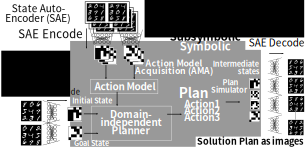
\includegraphics[width=\linewidth]{img/planning.pdf}
 \caption{Classical planning in latent space:
It uses the learned State AutoEncoder (\refig{sae}) to convert pairs of images $(\before,\after)$ to symbolic transitions,
 from which the Action Model Acquisition (AMA) component generates an action model.
A classical planner finds the symbolic solution plan for symbolic initial/goal states encoded from images.
Finally, intermediate states in the plan are decoded back to a human-comprehensible image sequence.}
\label{fig:overview}
\end{figure}

\latentplanner (\refig{fig:overview}) takes two inputs.
The first input is the \emph{transition input} $Tr$, a set of pairs of raw data.
Each pair $tr_i=(\before_i, \after_i) \in Tr$ represents a transition of the environment before and after some action is executed.
The second input is the \emph{planning input} $(i, g)$, a pair of raw data, which corresponds to the initial and the goal state of the environment.
The output of \latentplanner is a data sequence representing the plan execution that reaches $g$ from $i$.
While the original paper uses an image-based implementation (``data'' = raw images),
the type of data is arbitrary as long as it is compatible to neural network.

% Emphasize the type of symbol, as readers are not familier with or haven't deeply thought about symbols
% \subsection{SAE for Propositional Symbol Grounding}

\latentplanner works in 3 phases.
In Phase 1, a \emph{State AutoEncoder} (SAE) (\refig{sae}) learns a bidirectional mapping between raw data (subsymbolic representation e.g., images)
 and propositional states (symbolic representation) from a set of unlabeled, random snapshots of the environment.
% The $Encode$ function maps images to propositional states, and $Decode$ function maps the propositional states back to images:
The trained SAE provides two functions:
\begin{itemize} %this is crucial to understanding the rest of the paper, so making an itemize to highlight it
\setlength{\itemsep}{-0.3em}
\item $b=Encode(r)$ maps an image  $r$ to a boolean vector $b$.
\item $\tilde{r}=Decode(b)$ maps a boolean vector $b$ to an image $\tilde{r}$.
\end{itemize}
After training the SAE from $\braces{\before_i, \after_i\ldots}$,
it applies $Encode$ to each $tr_i \in Tr$ and obtain $(Encode(\before_i),$ $Encode(\after_i))=$ $(s_i,t_i)=$ $\overline{tr}_i\in \overline{Tr}$,
the symbolic representations (latent space vectors) of the transitions.

In Phase 2, an Action Model Acquisition (AMA) method learns an action model (e.g. PDDL, successor function) from $\overline{Tr}$ in an unsupervised manner.
The original paper proposed two approaches: AMA$_1$ is an oracular model which directly generates a PDDL without learning,
by allowing it to use the whole set of valid transitions as an oracle.
In contrast, AMA$_2$ is an unsupervised machine learning model that can learn from limited examples.

In Phase 3, a planning problem instance is generated from the planning input $(i,g)$.
These are converted to symbolic states by the SAE, and the symbolic planner solves the problem.
For example, an 8-puzzle problem instance consists of an image of the start (scrambled) configuration of the puzzle ($i$), and an image of the solved state ($g$).

Since the intermediate states comprising the plan are SAE-generated latent bit vectors, the ``meaning'' of each state (and thus the plan) is not clear to a human observer.
However, in the final step, \latentplanner obtain a step-by-step visualization of the plan execution
by $Decode$'ing the latent bit vectors for each intermediate state.
This necessitates the bidirectionality of the mapping between the input and the propositional states.

\begin{figure}[htb]
 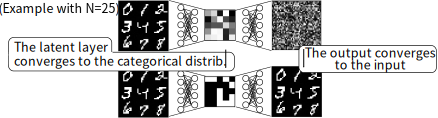
\includegraphics[width=\linewidth]{img/train-state-ae.pdf}
 \caption{Step 1:
Train the State AutoEncoder by
 minimizing the sum of the reconstruction loss and the variational loss of Gumbel-Softmax.
As the training continues, the output of the network converges to the input images.
Also, as the Gumbel-Softmax temperature $\tau$ decreases during training,
the latent values approach either 0 or 1.}
 % \caption{State AutoEncoder, a
 % Variational AutoEncoder \cite{kingma2014semi} using Gumbel-Softmax \cite{jang2016categorical} reparametrization in its
 % latent layer.}
 \label{sae}
\end{figure}

\subsection{SAE as a Variational AutoEncoder using Gumbel-Softmax}

The key concept of the SAE in \latentplanner is the use of Gumbel-Softmax \cite{jang2016categorical}
reparameterization trick in the latent activation of Variational AutoEncoder.
This allows SAE to obtain the
discretized binary representation, and \latentplanner uses this
discrete vector as the state representation for classical planning.

An AutoEncoder (AE) is a type of feed-forward neural network that learns
an identity function whose output matches the input \cite{hinton2006reducing}.
AEs are trained by backpropagation (BP) to minimize the reconstruction loss,
the distance between the input and the output according to a distance function such as Euclidean distance.
Since it is trained solely by the raw input data, it is a unsupervised learning method that do not require the human-assigned labels.
Its intermediate layer (typically smaller than the input) has a compressed, \emph{latent representation} of the input.
% AEs are commonly used for pretraining a NN.
NNs, including AEs, typically have continuous activations and integrating them with propositional reasoners is not straightforward.

A Variational AutoEncoder (VAE) \cite{kingma2013auto} is a type of AE that forces the \emph{latent layer} (the most compressed layer in the AE) to follow a certain distribution (e.g., Gaussian).
% While initially proposed for enforcing Gaussian distributions, VAEs have been used to enforce arbitrary types of distribution (notably by Generative Adversarial Network \cite{goodfellow2014generative,makhzani2015adversarial}). 
Since the random distribution is not differentiable (BP is not applicable), VAEs use \emph{reparameterization tricks}, which decompose the target distribution into a differentiable and a purely random distribution (the latter does not require the gradient).
For example, the Gaussian $N(\sigma,\mu)$ is decomposed to $\mu+\sigma N(1,0)$, where $\mu,\sigma$ are learned.
In addition to the reconstruction loss, VAE should also minimize the variational loss (the difference between the learned and the target distributions) measured by, e.g.,  KL divergence.

Gumbel-Softmax (GS) is a re\-para\-metri\-zation trick \cite{jang2016categorical} for categorical distribution.
It continuously approximates Gumbel-Max \cite{maddison2014sampling}, a method for drawing categorical samples.
Assume the output $z$ is a one-hot vector, e.g. if the domain is $D=\braces{a,b,c}$, $\brackets{0,1,0}$ represents ``b''.
The input is a class probability vector $\pi$, e.g. $\brackets{.1,.1,.8}$.
Gumbel-Max draws samples from $D$ following $\pi$:
% \[
 $z_i \equiv [ \text{if}\ i\ \text{is} \arg \max_j (g_j+\log \pi_j) \text{then}\ 1\ \text{else}\ 0 ]$
% \]
where $g_j$ are i.i.d samples drawn from Gumbel$(0,1)$ \cite{gumbel1954statistical}.
Gumbel distribution is a random distribution that can be sampled from $-\log (-\log (\text{Uniform}(0,1)))$, where
$\text{Uniform}(0,1)$ is a uniform random distribution between 0 and 1.
Gumbel-Softmax approximates argmax with softmax to make it differentiable:
% \[
$z_i = \text{Softmax}((g_i+\log \pi_i)/\tau)$.
% \]
``Temperature'' $\tau$ controls the magnitude of approximation, which is annealed to 0 by a certain schedule.
The output of GS converges to a discrete one-hot vector when $\tau\approx 0$.

In a vanilla SAE \cite{Asai2018}, there are $N$ units of Gumbel-Softmax
for $M=2$ categories in the latent layer, resulting in a $N\times 2$ matrix,
where $N$ specifies the number of propositional variables in the latent
state representation. The latent layer can be written as
$z_{ij}$ where $j\in \braces{0,1}$ and $1\leq i \leq N$.  When the
temperature $\tau$ is low, one of $z_{i0}$ or $z_{i1}$ takes the value
near 1 and another one takes the value near 0 (one-hot vector).  A binary
propositional vector $b$ can thus be extracted by taking the first row, i.e.,
$b=\parens{b_1\ldots b_N}=\parens{z_{10}\ldots z_{N0}}$.

\subsection{AMA$_1$, an Oracular Action Model Acquisition method}

Action Model Acquisition method AMA$_1$ produces a PDDL/SAS model compatible to
FastDownward \cite{Helmert04}, but is an oracular model which requires the entire state transitions
in the environment.
For each pair of observations $\parens{\before_i, \after_i}$ in the entire set of state transitions allowed in the environment,
AMA$_1$ uses SAE to encodes it into 
a symbolic transition $(Encode(\before_i),$ $Encode(\after_i))=$ $(s_i,t_i)$ where $s_i,t_i$ are propositional states.
Each state (either $s_i,t_i$) is represented as a binary vector $(b_j)_{1\leq j \leq N}$.
Each symbolic transition is then encoded into a PDDL action 
using $s_i$ as its preconditions and the difference of $s_i$ and $t_i$ as its effects.
Each bit $b_j$ is converted into zero-ary predicate \texttt{($b_j$-true)} and \texttt{($b_j$-false)}
when $b_j=1$ and $0$, respectively.
For instance, when $b_5$ is 0 in $s_i$ and 1 in $t_i$,
the preconditions include \texttt{(b5-false)} and
the effects include \texttt{(and (not (b5-false)) (b5-true))}.

\subsection{Regularization in Neural Network}

\emph{Regularization} is an important and broad concept in machine learning
that limits the representation capacity of a machine learning model by adding a constraint,
so that the model better adapt to the underlying characteristics of the dataset.
Regularization trades the (training) performance with generalization capability (testing performance, robustness to
unseen data points) in order to suppress overfitting.
Regularization could be implemented in various ways.

One way is to organize and restrain the network connection for the particular data,
such as Convolutional Networks for images
or Recurrent Networks for sequential data, or
Dropout \cite{srivastava2014dropout}, that randomly drops some neurons so
that each pattern is more strongly associated with a fewer set of nodes.

Another way is to add a penalty term to the optimization metric of the
neural network that is minimized by algorithms like Stochastic
Gradient Descent.
Common regularization techniques in this category include
$l_1$ (LASSO) or $l_2$ regularization that penalize the absolute sum / square sum of the
activations.

% It is necessary for the mapping to be bidirectional, because the
% propositional variables are machine-generated symbols, and also the
% resulting plan (returned as a sequence of propositional states) should
% be decoded back to real-world images which are interpretable for humans.

% \latentplanner also learns the action model using a neural action model acquisition method AMA$_2$,
% but we omit the details due to space limitation.

\section{Symbol Stability Problem}
% \section{Issues in the State Representation\\ in the Vanilla SAE}
\label{issues}

SAE in \latentplanner can map a visual observation of the environment to/from a set of propositional values.
An issue in a vanilla SAE is that the class probability that is used inside its Gumbel-Softmax could be
neutral for the class ``true'' and the class ``false'', and the resulting value
of a proposition is random (\refig{unstable}).
The randomness of the vanilla SAE comes from the way
Gumbel distribution is sampled, $-\log (-\log (\text{Uniform}(0,1)))$, which includes
a uniform random distribution.
This causes several problems from the classical planning point of view.

\begin{figure}[htb]
 \centering
 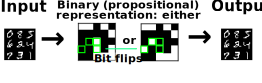
\includegraphics{img/unstable.pdf}
 \caption{Propositions found by Vanilla SAE may contain several uninformative bits
 that flip randomly and do not affect the output.}
 \label{unstable}
\end{figure}

First, search algorithms that run on the state space generated based on these propositional vectors
are confused by many variation of the essentially identical real world states.
It could visit several variations of the same real world state that are encoded into different propositional vectors,
however the duplicate detection in state space search algorithms (e.g. \astar) treat them as separate states.
% since it completely relies on the atomiticy and deteminisim of the proposition.
This slows down the search by increasing the number of nodes that can be reachable from the initial state.

\begin{figure}[htb]
 \centering
 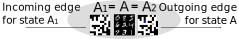
\includegraphics{img/disconnected.pdf}
 \caption{Random variations of propositional encoding for a single real-world state could disconnect the search space.}
 \label{disconnected}
\end{figure}

Secondly, the state space could be disconnected due to such random variations (\refig{disconnected}).
Some states may be reached only via a single variation of the real world state, and is not connected to the
other variation of the propositional state that represents the same real-world state.
In fact, in the appendix section in the Arxiv version of the original paper \cite{Asai2018},
the authors stated that they used \emph{state augmentation} technique
which circumvent this problem by sampling states from the same image multiple times.

Thirdly, in order to reduce the stochasticity of the propositions we encounter a hyperparameter tuning problem
which is costly when we train a large neural network.
We note that while some values in the latent layer are random, most of values are not.
These unused, uninformative bits are generated because the network has an excessive capacity to 
model the entire state space, i.e. they appear when we specify the number of proposition $N$ too large.
If we decrease $N$ while maintaining the reconstruction capability of the SAE, the number of uninformative bits
reduces.
On the contrary, if we specify $N$ too small, it lacks the capacity to represent the state space
and the SAE is no longer able to reconstruct the
real world image.
As a result, we face a hyperparameter tuning problem: Too large $N$ causes a disconnected/bloated state space graph,
and too small $N$ does not converge on the dataset.

% \section{Symbol Stability Problem}

As we have seen, unstable propositional representations are harmful for symbolic reasoning algorithms (search)
in various ways.
Fundamentally,
these harmful effects are caused by breaking a critical feature of a symbol, \emph{designation} \cite{newell1976computer,newell1980physical},
that each symbol uniquely refers to an entity (referent, concept, meaning).
If a meaning of a symbol changes frequently and in an unexpected manner, the entire symbolic manipulation is fruitless
because the underlying symbols are not grounded / tied to a particular concept, and does not represent the real world.

[more intuitive example?]
% A famous 
% Colorless green ideas sleep furiously

Thus, a symbol grounding procedure should not only find \emph{some} set of symbols that is sufficient to represent the
environment, but also find a \emph{stable} symbolic representation that uniquely describes the environment.
% This stability should be checked 

\begin{defi}
A \emph{symbolic representation} of an environment is a set of symbols
whose referents can reconstruct the environment with a certain function with a sufficient accuracy.
\end{defi}

\begin{defi}
A symbol in a symbolic representation of an environment is \emph{stable}
when its referent (e.g. truth assignment for propositional symbols) is identical
for the same observation of the environment that is represented.
\end{defi}

From a practical perspective, 
the impact of unstable symbols on symbolic reasoning systems is typically exponential to the number of unstable symbols.
For example, in the case of search algorithms, each unstable symbol doubles the size of the state space (being true or false).
% In a hypothetical Prolog-like logic programming system, each unstable predicate symbol would also double the
% number of unifications.



% stability

The stability of the representation obtained by a neural network depends
on whether the network contains stochasticity during runtime.
% 
In other words, any stochastic symbol grounding system potentially suffers from 
the symbol stability problem.
% 
In recent years,
an increasing number of neural networks relies on some form of random
sampling processes.  VAE family of networks
\cite{kingma2013auto,jang2016categorical,higgins2016beta},
contains a source of stochasticity in the network. Generative
Adversarial Networks \cite[GAN]{goodfellow2014generative} also samples
the latent space to generate the real-world data.

% \section{Zero-Suppressed State AutoEncoder (ZSAE) and Entropy-Minimizing State AutoEncoder (ESAE)}
\section{Zero-Suppressed State AutoEncoder (ZSAE)}
\label{zsae}

To tackle the symbol stability problem in Latplan, we propose Zero-Suppressed State AutoEncoder (ZSAE),
a SAE with a additional regularization mechanism which is simple but efficient.
The basic idea for our additional regularization is simple: Just penalize the
1-bit in the latent layer, so that no propositions unnecessarily flip to true at random,
while preserving the propositions that are absolutely necessary for representing the reconstruction accuracy.
Since Gumbel-Softmax (GS) is basically a Softmax function,
and SAE uses 2 categories, this can be seen as adding an
asymmetric penalty for a particular class label used in the encoding.

The resulting loss function below is similar to the $l_1$ norm (LASSO) typically
applied to continuous activation values:
\begin{align*}
 \brackets{\text{loss}} = & \brackets{\text{\small Reconstruction}} &+ & \brackets{\text{\small GS loss}} &+ & \brackets{\text{\small 0-Sup. loss}} \\ 
 % =                      & D_\text{KL}(r || \tilde{r}) &+ & \text{mean}(q \log Mq)           &+ & \alpha \text{mean}(b)              \\
 =                        & \text{BCE}(r,\tilde{r})     &+ & \text{mean}(q \log Mq)           &+ & \alpha \text{mean}(b)
\end{align*}
where BCE stands for Binary Cross Entropy loss,
$M=2$, $q=\text{Softmax}(\log \pi_i)$ and $\log \pi_i$ is the un-normalized input logit to Gumbel-Softmax.
$\alpha$ is a hyperparameter which specifies the magnitude of the zero-suppression.
Similar to $l_1$ regularization, this achieves a sparser representation in the binary domain where
 more propositions take the value of 0 (\refig{zsae-overview}).

One additional advantage of applying $l_1$ norm is that, when the representation becomes deterministic,
several neurons are completely deactivated, i.e. always takes the value of zero
and can be pruned afterwards to reduce the network size.

A possible interpretation of this approach from the symbolic perspective is that
this $l_1$ (LASSO) regularization is working as a prior representing \emph{closed-world assumption} \cite[CWA]{reiter1981closed}.
CWA is an assumption that all propositions take the value \texttt{false}
when they are unknown to a Knowledge Base (KB) or cannot be proven from it (negation as failure).
% [wrong!]
% We could interpret these unknown propositions defaulted to be false as those which are irrelevant
% to the current task that the agent is solving.
Being always false, the agent can safely ignore them because
they do not initiate an additional set of rules in the rule database by satisfying further preconditions.
Also, the KB enjoys the space reduction for storing facts
because it does not have to explicitly store the false propositions.

In our Zero-Suppressed SAE, nodes that do not affect the output are stabilized to zero
and can be safely pruned.
Moreover, we could conceive that there are infinite number of propositions
that are already pruned from the network and are just invisible, just as all unknown propositions
are regarded as false and need not be explicitly saved in the Knowledge Base.
In other words, combining discrete representation and zero-suppression,
ZSAE embeds closed-world assumption in the network as a model prior.


\section{Empirical Evaluation}
\label{evaluation}

We tested the vanilla SAE and the Zero-suppressed SAE across 5 different
image domains depicting 8-puzzles or Lights Out puzzle game \cite{lightsout}.

\textbf{MNIST 8-puzzle}
is an image-based version of the 8-puzzle, where tiles contain hand-written digits (0-9) from the  MNIST database \cite{lecun1998gradient}.
Valid moves in this domain swap the ``0'' tile  with a neighboring tile, i.e., the ``0'' serves as the ``blank'' tile in the classic 8-puzzle. 
The \textbf{Scrambled Photograph 8-puzzle (Mandrill, Spider)} cuts and scrambles real photographs, similar to the puzzles sold in stores).
These differ from the MNIST 8-puzzle in that ``tiles'' are \textit{not} cleanly separated by black regions
(we re-emphasize that \latentplanner has no built-in notion of square or movable region).
% In \textbf{Towers of Hanoi (ToH)},
% we generated the 4 disks instances.
% 4-disk ToH resulted in a 15-step optimal plan.
\textbf{LightsOut} is
a video game where a grid of lights is in some on/off configuration ($+$: On),
and pressing a light toggles its state as well as the states of its neighbors.
The goal is all lights Off.
Unlike previous puzzles, a single operator can flip 5/16 locations at once and
removes some ``objects'' (lights).
This demonstrates that \latentplanner is not limited to domains with highly local effects and static objects.
\textbf{Twisted LightsOut} distorts the original LightsOut game image by a swirl effect, 
showing that \latentplanner is not limited to handling rectangular ``objects''/regions.

Each domain has 60 problem instances each generated by a random walk from
the goal state. 60 instances consists of 30 instances each generated by a 7-steps random walk
and another 30 by 14 steps. 30 instances consists of 10 instances whose images are corrupted by gaussian noise,
10 with salt/pepper noise and another 10 with no noise.

% There are three versions of 8-puzzles (MNIST, Mandrill, Spider).
% MNIST 8-puzzle is an image-based versions of the 8-puzzle, where tiles contain
% hand-written digits (0-9) from the MNIST database
% \cite{lecun1998gradient}. Each digit is shrunk to 14x14 pixels, so each
% state of the puzzle is a 42x42 image.  Valid moves in this domain swap
% the ``0'' tile with a neighboring tile, i.e., the ``0'' serves as the
% ``blank'' tile in the classic 8-puzzle.  The entire state space consists
% of 362880 states ($9!$) and 967680 actions.  From any specific goal state, the reachable
% number of states is 181440 ($9!/2$).  Note that the same image is used
% for each digit in all states, e.g., the tile for the ``1'' digit is the
% same image in all states.
% 
% Mandrill and Spider are 8-puzzles generated by cutting and scrambling real photographs
% (similar to sliding tile puzzle toys sold in stores). We used the
% ``Mandrill'' and ``Spider'' images, two of the standard benchmark in the image processing
% literature.  The image was first converted to greyscale and then
% % rounded to black/white (0/1) values
% histogram-normalization and contrast enhancement was applied.
% The same number of transitions as in the MNIST-8puzzle experiments are used.
% 
% 
% Lights Out is a puzzle game where a grid of lights is in some on/off configuration ($+$: On),
% and pressing a light toggles its state (On/Off) as well as the state of all of its neighbors.
% The goal is all lights Off.
% The image dimension is 36x36 and the size of each button ($+$ button) is 9x9.
% 4x4 LightsOut has $2^{16}=65536$ states and $16\times 2^{16}=1048576$ transitions.
% Similar to the 8-puzzle instances, we used 20000 transitions.
% Training:validation ratio 9:1 is maintained (i.e. only 36000 images and 18000 transitions are used for training).
% 
% Another version of Lights Out game is Twisted LightsOut.
% While the images have the same structure as LightsOut, 
% we additionally applied a swirl effect available in scikit-image package
% in order to remove the grid-like structure in the images.
% The effect is applied to the center, with strength=3, linear interpolation, 
% and radius equal to 0.75 times the dimension of the image.
\subsection{State Variance}


\begin{table*}[htbp]
 \relsize{-1}
 \centering
 \setlength{\tabcolsep}{0.45em}
 \begin{tabular}{|r|*{3}{*{6}{c|}}}
     & \multicolumn{6}{c|}{Max. variance over bits}
     & \multicolumn{6}{c|}{True ratio}
     & \multicolumn{6}{c|}{Effective bits}
     % & \multicolumn{6}{c|}{Mean Square Error}
  \\
$N=$ & \multicolumn{3}{c|}{100} & \multicolumn{3}{c|}{1000}
     & \multicolumn{3}{c|}{100} & \multicolumn{3}{c|}{1000}
     & \multicolumn{3}{c|}{100} & \multicolumn{3}{c|}{1000}
     % & \multicolumn{3}{c|}{100} & \multicolumn{3}{c|}{1000}
  \\
$\alpha=$   & 0 (SAE) &  0.2  &  0.7   & 0 (SAE) &  0.2   &  0.7   & 0 (SAE) &  0.2  &  0.7   & 0 (SAE) &  0.2   &  0.7   &  0   &  0.2 &  0.7  & 0 (SAE) &  0.2   &  0.7   \\% & 0 (SAE) &  0.2  &  0.7   & 0 (SAE) &  0.2   &  0.7   \\
MNIST       &  0.21   &  0.03 &  0.14  &  0.22   &  0.17  &  0.18  &  0.50   &  0.20 &  0.13  &  0.49   &  0.06  &  0.02  &  100 &  41  &  42   &  1000   &  119   &  46    \\% &  0.00   &  0.00 &  0.00  &  0.00   &  0.00  &  0.00  \\
Mandrill    &  0.21   &  0.00 &  0.07  &  0.22   &  0.11  &  0.21  &  0.49   &  0.45 &  0.17  &  0.50   &  0.48  &  0.03  &  100 &  90  &  37   &  1000   &  956   &  151   \\% &  0.00   &  0.00 &  0.00  &  0.00   &  0.00  &  0.00  \\
Spider      &  0.20   &  0.09 &  0.16  &  0.21   &  0.23  &  0.17  &  0.50   &  0.47 &  0.17  &  0.50   &  0.44  &  0.04  &  100 &  94  &  43   &  1000   &  920   &  77    \\% &  0.00   &  0.00 &  0.00  &  0.00   &  0.00  &  0.00  \\
% LightsOut &  0.21   &  0.09 & (0.21) &  0.20   &  0.21  &  0.20  &  0.50   &  0.41 & (0.43) &  0.50   &  0.46  &  0.04  &  100 &  82  & (100) &  1000   &  921   &  492   \\% &  0.00   &  0.00 & (0.01) &  0.00   &  0.00  &  0.00  \\
% Twisted   &  0.20   &  0.17 & (0.22) &  0.22   &  0.21  & (0.22) &  0.51   &  0.37 & (0.89) &  0.50   &  0.50  & (0.50) &  100 &  73  & (98)  &  1000   &  998   & (1000) \\% &  0.00   &  0.00 & (0.08) &  0.00   &  0.00  & (0.03) \\
% Hanoi     &  0.18   &  0.16 & (0.17) & (0.20)  & (0.19) & (0.20) &  0.50   &  0.44 & (0.96) & (0.50)  & (0.48) & (0.69) &  100 &  100 & (100) & (1000)  & (1000) & (1000) \\% &  0.00   &  0.00 & (0.37) & (0.02)  & (0.01) & (0.28) \\
% LightsOut &  0.21   &  0.09 & -      &  0.20   &  0.21  &  0.20  &  0.50   &  0.41 & -      &  0.50   &  0.46  &  0.04  &  100 &  82  & -     &  1000   &  921   &  492   \\% &  0.00   &  0.00 & -      &  0.00   &  0.00  &  0.00  \\
% Twisted   &  0.20   &  0.17 & -      &  0.22   &  0.21  & -      &  0.51   &  0.37 & -      &  0.50   &  0.50  & -      &  100 &  73  & -     &  1000   &  998   & -      \\% &  0.00   &  0.00 & -      &  0.00   &  0.00  & -      \\
% Hanoi     &  0.18   &  0.16 & -      & -       & -      & -      &  0.50   &  0.44 & -      & -       & -      & -      &  100 &  100 & -     & -       & -      & -      \\% &  0.00   &  0.00 & -      & -       & -      & -      \\
LightsOut   &  0.21   &  0.09 & -      &  0.20   &  0.21  &  0.20  &  0.50   &  0.41 & -      &  0.50   &  0.46  &  0.04  &  100 &  82  & -     &  1000   &  921   &  492   \\% &  0.00   &  0.00 & (0.01) &  0.00   &  0.00  &  0.00  \\
Twisted     &  0.20   &  0.17 & -      &  0.22   &  0.21  & -      &  0.51   &  0.37 & -      &  0.50   &  0.50  & -      &  100 &  73  & -     &  1000   &  998   & -      \\% &  0.00   &  0.00 & (0.08) &  0.00   &  0.00  & (0.03) \\
% Hanoi       &  0.18   &  0.16 & -      & -       & -      & -      &  0.50   &  0.44 & -      & -       & -      & -      &  100 &  100 & -     & -       & -      & -      \\% &  0.00   &  0.00 & (0.37) & (0.02)  & (0.01) & (0.28) \\
\end{tabular}
 \caption{Results comparing the characteristics of Vanilla SAE (ZSAE with $\alpha=0$) and ZSAE with various $\alpha$,
 over 100 randomly generated images encoded 100 times.
 $\alpha=0$ means the vanilla SAE without zero suppression.
 Results are not shown when the neural network failed to converge (Mean square error between the input and the output larger than 0.01).
 }
\label{tab:stability}
\end{table*}



We first tested the variance or randomness of the state encoding between
the original SAE (pure Gumbel-softmax latent layer) and the ZSAE with various $\alpha$.
We randomly generated 100 images with a domain-specific generator for each puzzle domain,
then encoded them with Z/SAE 100 times.
We measured the variance of the latent layer, i.e. the variance of latent activations (0 or 1)
across 100 encoding trials of the same image.
We took the maximum variance over the entire propositions and 100 input images.
\reftbl{tab:stability} (first columns) shows that the propositions made by Vanilla SAE are highly random,
while additional regularization in ZSAE suppresses the stochastic behavior
and achieves a stable propositional representation.

We next measured the average percentage of propositions that turned true.
\reftbl{tab:stability} (middle columns) shows that the ratio significantly drops due to the Zero-suppression penalty.

Finally, \reftbl{tab:stability} (right columns) shows that the number of effective bits,
i.e. the number of propositions that \emph{ever} turned true, is low in ZSAE.
In MNIST, the numbers are comparable between ZSAEs with $(N,\alpha)=(100,0.7)$ and $(1000,0.7)$.
This shows that the network can sometimes find an encoding of almost the same size
regardless of the size of the latent layer (upper bound of the size of
propositions). The additional
penalty encourages the network to find the more compact representation,
rather than freely consuming the latent space capacity in an entangled representation.

% Furthermore, while regularization in general tends to trade accuracy and
% the desired characteristics in the activation, we observe that the
% reconstruction loss is still low if you maintain the latent space size
% large enough.

\subsection{Planner Performance}

Next we compared the success ratio of \latentplanner using Z/SAE with various parameters.
We tested both Action Model Acquisition (AMA) methods AMA$_1$ and AMA$_2$ proposed in \cite{Asai2018}.

We first tested AMA$_1$, an oracular, idealistic AMA that does not incorporate machine learning,
and instead generates the entire propositional state transitions from the entire image transitions.
The purpose we test an impractical AMA$_1$ methods is
to separate the effect of a better state representation achieved by ZSAE
and that of the learning procedure in AMA$_2$ that learns the state transitions and action rules.
The results in \reftbl{tab:ama1} shows that ZSAE achieves the overall improvement in terms of success ratio.

\begin{table}[htbp]
\centering
% \relsize{-1}
\begin{tabular}{r|rrr|rrr}
 & \multicolumn{3}{c|}{SAE} & \multicolumn{3}{c}{ZSAE ($\alpha=0.2$)} \\ 
$N=$           & {36}        & {64}        & {100} & {36}        & {64}        & {100}        \\\hline
Digital        & \textbf{60} & 59          & 49    & \textbf{60} & 59          & 59           \\
Mandrill       & 58          & 58          & 15    & \textbf{60} & \textbf{60} & \textbf{60}  \\
MNIST          & \textbf{57} & 25          & 15    & 49          & 50          & \textbf{57}  \\
Spider         & 0           & \textbf{60} & 56    & 42          & \textbf{60} & \textbf{60}  \\
Twisted        & \textbf{60} & 58          & 35    & \textbf{60} & \textbf{60} & \textbf{60}  \\\hline
\textbf{Total} & {235}       & {260}       & {170} & {271}       & {289}       & \textbf{296} \\
\end{tabular}
\caption{Results using AMA$_1$ (oracular method) for comparing the performance of Z/SAE.
AMA$_1$ is not a learning-based action model acquisition method, therefore SAE implementation does not affect its performance.
Best results in each domain are highlighted in \textbf{bold}.
Results indicates that ZSAE is more robust on different hyperparameters and tend to achieve better performance than vanilla SAE.
SAE performance is sometimes comparable to ZSAE but only when it is tuned appropriately.
}
\label{tab:ama1}
\end{table}

Another harmful effect of unstable propositions is
its effect on the duplicate detection mechanism in search algorithms.
To demonstrate that this effect is also suppressed by ZSAE,
we measured the number of node generation
on models generated by Vanilla SAE and ZSAE and successfully solved by
the planner (\refig{fig:ama1-visited}).
% ???
% Since the planner uses a blind search and the problem is unit-cost, all nodes under the solution depth are generated
% (note: mind the difference between evaluation, expansion, generation).
The plot supports our claim that
the randomness in the state encoding of Vanilla SAE confuses the duplicate detection and
generates larger number of states compared to ZSAE.

\begin{figure}[htb]
 \centering
 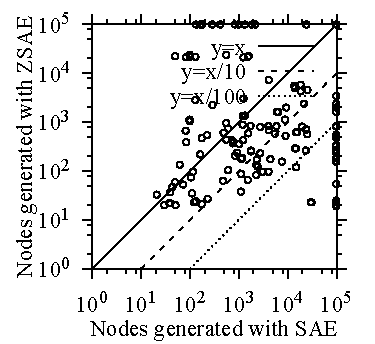
\includegraphics{img/static/gen.pdf}
 \caption{Double-logarithmic plot of the number of states generated by blind search
for the search space obtained from SAE and ZSAE with $N=64,100$. 
Unsolved instances are shown on the borders, indicating planning with vanilla SAE fails more often than in ZSAE.
 % 
We observe that planning under SAE-generated search space could generate x100 more states
than under ZSAE-generated search space, while the opposite happens only up to x5 more states.
The latter case happens due to the difference in the tiebreaking orders and also because some nodes randomly become unreachable (disconnected) in SAE.
$N=36$ is not shown because
it is a parameter tuned for SAE to have stable propositions, thus the comparison does not make sense.
}
 \label{fig:ama1-visited}
\end{figure}

Next, we show the performance when AMA$_2$ is used
(\reftbl{tab:ama2}). Networks in AMA$_2$ (AAE/AD/SD) are trained with the same hyperparameter 
used in the original paper \cite{Asai2018}.
Similar results were obtained; ZSAE consistently improves the success ratio.

\begin{table}[htb]
 \vspace{1.5in}
 \caption{}
 \label{tab:ama2}
\end{table}

To identify the reason of the improvement, we measured the State / Action Discriminator accuracy in those domains.
From \refig{fig:ama2-ad}, we observe the accuracy was improved by the ZSAE.

\begin{figure}[htb]
 \vspace{1.5in}
 \caption{State Discriminator / Action Discriminator accuracy between ZSAE and SAE.}
 \label{fig:ama2-ad}
\end{figure}

\subsection{Pruning Inactive Nodes from ZSAE}

[too obvisous and intuitive?]

We compute the amount of memory reduction possible by the pruning on the nodes
that has a constant activation of 0. As we saw from \reftbl{tab:stability},
Vanilla SAE does not have such propositions (all bits are effective bits).
% While we did not actually implemented the node pruning,

First, since our network has a fully-connected network between the
latent layer and the convolutional layer before it, node reduction
amounts to quadratic weight reduction.  Representing a fully-connected
network between two layers of $L$ and $N$ nodes requires $(L+1)N$
weights ($+1$ for the bias).
In the network we used, $L=1000$. Thus, in the case of ZSAE with $\alpha=0.7, N=1000$
where it reduces the representation down to only 46 effective bits, weights are reduced by 954954,
which is huge compared to the convolutional weights (3x3, 16 channels, thus 144 float values).
We do not show the entire results due to space limitation and also because the results are straightforward.

Second, we considered the inference time by the number of multiplication operations and also by the actual test.
First, the operations: In the same example above,
matrix multiplication $y=Wx+b$ (where $W$ is the weights and $b$ the bias) requires $LN$ multiplication and $L+N$ additions.
Moreover, the Gumbel-Softmax operation requires $N$ softmax calculations, gumbel sampling (two logarithms) and one float division.
This overall amounts to a linear speed up along the reduction of $N$, 
since the cost of addition is negligible to the cost of multiplication.

% \section{Declarative Knowledge Base based on ZSAE}
% 
% Since the ZSAE achieves a sparse encoding where the unused propositions
% tend to become false, the network has a large amount of unused weights
% which, if retrained properly, could be used for storing additional
% information that is provided afterwards, making the entire network looks
% like a declarative knowledge base where you can incrementally store
% new knowledge.
% 
% We verify this hypothesis by first training a ZSAE with some dataset, retraining the same ZSAE with
% a completely new dataset, then finally test the reconstruction accuracy for both dataset.

\section{Related Work}

% GS autotuning

We showed that $l_1$ regularization reduces the variance of the discrete
representation which resulted from the Gumbel random distribution
in Gumbel-Softmax reparameterization
trick.  A line of work that could introduce confusion might be REBAR
\cite{TuckerMMLS17}, an improvement to Gumbel-Softmax that automatically
adjusts the temperature parameter $\tau$ instead of using a fixed
schedule and achieves ``low-variance, unbiased gradient estimates'',
meaning that the training is more stable. The variance mentioned in
REBAR is the variance of the gradient estimates used during training, not the
resulting representation.

% declarative kb

% neural TM

% other regularization

$l_1$ (LASSO) regularization is a standard approach in the field of machine learning for improving the
generalization performance.
It is commonly applied to the network \emph{weight}, not activations,
thus has not been associated with the stability of the representation.
It has not been explicitly associated with the concept of
closed-world assumption, nor discussed in the context of symbol grounding.

Autoencoders with $l_1$ regularization applied on the hidden layer
is called sparse autoencoder \cite{ng2011cs294a}.
As a Deep-Learning practice,
this is useful for training an overcomplete network that has a larger latent space and smaller average activation.
The focus of the previous work in this direction aims at improving the testing accuracy and interpretability.
Also, previous work uses continuous and deterministic neural network that does not have stochasticity.
In contrast, the purpose of zero-suppression is to reduce the randomness of the representation
when the network contains stochasticity and the same testing accuracy should be maintained.

From another practical point of view from the data science,
$l_1$ regularization is considered in the context of feature selection for supervised learning,
where it is important to drop some data columns as unrelated.
This is a supervised learning setting, and the aim is to improve the classification performance.

% In a bio-inspired view, sparce coding is supposed to be natural since
% the neurons can fire less frequently and is energy efficient. [remove?]

In the literature of theoretical analysis of machine learning and generalization,
regularization in general are regarded as trading the bias and variance.
For example, $l_1$ regularization applied on the hidden layer biases the representation toward 0 and decreases the variance.
However, this bias and variance are defined over the dataset \cite{deeplearningbook},
not the single data point as we discussed in this paper.
% 
Therefore, the variance in the typical context of machine learning and the variance of the latent representation
for a single data point that we discussed in this paper are orthogonal.

% While an asymmetric penalty may seem unintuitive, this is a common
% strategy particularly in Zero-Suppressed Binary Decision Diagram (ZDD)
% \cite{minato1993zero}, a type of binary decision diagram \cite{bryant1986graph} which
% uses an asymmetric rule for pruning decision nodes, achieving a greater
% performance over BDD in representing a sparse, ``almost zero'' binary dataset.

% ZDDs can efficiently represent a set of subsets e.g. $\braces{\braces{a,c},\braces{b,c}}$.
% The reduction rule of ZDDs can prune the nodes for items that never appear in the subsets.
% For instance, an item $d$ does not belong to any of the subsets shown above, therefore $d$ does not have
% a corresponding decision node in the diagram.
% While potentially there could be an infinite number of items in the environment, they are 
% all irrelevant to the above set and therefore pruned from the diagram.

% Another, rather non-intuitive topic related to the sparser binary representation
% is the connection to \emph{close-world assumption} \cite{reiter1981closed}, which assumes all unknown
% propositions to be false.
% % 
% We could interpret these unknown propositions defaulted to be false as those which are irrelevant
% to the current task that the agent is solving.
% Being always false, the agent can safely ignore them because
% they do not initiate an additional set of rules in the rule database by satisfying further preconditions.
% 
% % 
% Similarly, in our Zero-Suppressed SAE, not only nodes that do not affect the output are stabilized to zero
% and can be safely pruned, but also we could conceive that there are infinite number of propositions
% that are already pruned from the network and are just invisible.
% In other words, combining discrete representation and zero-suppression,
% ZSAE embeds closed-world assumption in the network as a model prior.

% [TODO: more on Binarized NN]

Binarized Neural Networks \cite{courbariaux2015binaryconnect,HubaraCSEB16,rastegari2016xnor}
 are implementation methods of NNs designed for
memory-limited embedded applications or FPGAs. They constrain the weights and/or activation
values to $\braces{-1,+1}$ and perform the forward/backward processes of NN using
efficient binary operations such as XNOR and popcount.
To our knowledge, there is no $l_1$-based regularization successfully
applied to binarized networks, while the use of Dropouts, Batch Normalization, 
or noisy weights \cite{HubaraCSEB16} are common.
However, note that activations in SAE are binarized only in the latent layer,
and they are not binarized from the beginning of training
 as in the case of binarized networks, and that weights are not binarized at all.
The purpose of implementing a binary representation is also different, where BNNs
are aimed at memory usage and low-level performance while SAE aims at symbolic computation.

\section{Conclusion}
\label{conclusion}

We introduced Zero-Suppressed State AutoEncoder (ZSAE), inspired from
Zero-Suppressed Decision Diagram, which addresses an issue in the state
encoding made by \latentplanner, improves its performance, removes the need
for aggressive hyperparameter tuning as well as achieves a
neural-symbolic declarative knowledge base.  The ZSAE improves upon the
regular State AutoEncoder (SAE) proposed by \citeauthor{Asai2018} by
adding an asymmetric penalty similar to $l_1$ regularization to the optimization metric of
Neural Network, which tries to minimize the number of true propositions
when encoding a raw state input such as images.

% ?
A promising direction for future work is to build a first-order logical
representation of the input domain building upon \latentplanner system.

